\let\negmedspace\undefined
\let\negthickspace\undefined
\documentclass[journal,12pt,onecolumn,article]{IEEEtran}
\usepackage{cite}
\usepackage{color,soul}
\usepackage{amsmath,amssymb,amsfonts,amsthm}
\usepackage{algorithmic}
\usepackage{graphicx}
\usepackage{textcomp}
\usepackage{xcolor}
\usepackage{subcaption}
\usepackage{txfonts}
\usepackage{listings}
\usepackage{enumitem}
\usepackage{mathtools}
\usepackage{gensymb}
\usepackage{comment}
\usepackage[breaklinks=true]{hyperref}
\usepackage{tkz-euclide} 
\usepackage{listings}
\usepackage{multicol}
\usepackage{gvv}       
\usepackage[dvipsnames]{xcolor}
\def\inputGnumericTable{}                                
\usepackage[latin1]{inputenc}                            
\usepackage{color}                                       
\usepackage{array}                                       
\usepackage{longtable}                                   
\usepackage{calc}                                        
\usepackage{multirow}                                    
\usepackage{hhline}                                      
\usepackage{ifthen}                                      
\usepackage{lscape}
\usepackage{float}
\newtheorem{theorem}{Theorem}[section]
\newtheorem{problem}{Problem}
\newtheorem{proposition}{Proposition}[section]
\newtheorem{lemma}{Lemma}[section]
\newtheorem{corollary}[theorem]{Corollary}
\newtheorem{example}{Example}[section]
\newtheorem{definition}[problem]{Definition}
\newcommand{\BEQA}{\begin{eqnarray}}
\newcommand{\EEQA}{\end{eqnarray}}
\newcommand{\define}{\stackrel{\triangle}{=}}
\theoremstyle{remark}
\newtheorem{rem}{Remark}
\begin{document}
\bibliographystyle{IEEEtran}
\vspace{3cm}
\title{Gate-ASSIGNMENT-3}
\author{EE24BTECH11043 - Murra Rajesh Kumar Reddy}
\maketitle
\bigskip
\begin{enumerate}
	\item Which one of the following is a solution of $\frac{d^2 u\brak{x}}{dx^2}=k^2u\brak{x}$, for k real?
		\begin{enumerate}
			\item $e^{-kx}$
			\item $\sin {kx}$
			\item $\cos {kx}$
			\item $\sinh {x}$
		\end{enumerate}
	\item A real, invertible $3\times 3$ matrix M has eigenvalues $\lambda,\brak{i=1,2,3}$ and the corresponding eigenvectors are $|e_i\rangle , \brak{i=1,2,3}$ respectively. Which one of the following is correct?
		\begin{enumerate}
			\item $M |e_i \rangle = \frac{1}{\lambda_i}|e_i\rangle$, for $i=1,2,3$
			\item $M^{-1}|e_i \rangle = \frac{1}{\lambda_i}|e_i\rangle$, for $i=1,2,3$
			\item $M^{-1}|e_i \rangle = \lambda_i|e_i\rangle$, for $i=1,2,3$
			\item The eigenvalues of $M$ and $M^{-1}$ are not related.
		\end{enumerate}
	\item A quantum particle is subjected to the potential \\
		$ V\brak{x} =
		\begin{cases}
			\infty, & x\le -\frac{a}{2} \\
			0, & -\frac{a}{2} < x < \frac{a}{2} \\
			\infty, & x\ge \frac{a}{2}
		\end{cases}$ \\
		The ground state wave function of the particle is proportional to
		\begin{enumerate}
			\item $\sin{\brak{\frac{\pi x}{2a}}}$
			\item $\sin{\brak{\frac{\pi x}{a}}}$
			\item $\cos{\brak{\frac{\pi x}{2a}}}$
			\item $\cos{\brak{\frac{\pi x}{a}}}$
		\end{enumerate}
	\item Let $\hat{a}$ and $\hat{a}^{+}$, respectively denote the lowering and raising operators of a one-dimensional simple harmonic oscillator. Let $|n\rangle$ be the energy eigenstate of the simple harmonic oscillator. Given that $|n\rangle$ is also an eigen state of $\hat{a}^{+}\hat{a}^{+}\hat{a}\hat{a}$ , the corresponding eigenvalue is
		\begin{enumerate}
	\item $n\brak{n-1}$
	\item $n\brak{n+1}$
	\item $\brak{n+1}^2$
	\item $n^2$
		\end{enumerate}
	\item Which one of the following is a universal logic gate?
		\begin{enumerate}
			\item AND
			\item NOT
			\item OR
			\item NAND
		\end{enumerate}
	\item Which one of the following is the correct binary equivalent of the hexadecimal $F6C$ ?
		\begin{enumerate}
			\item 0110 1111 1100 
			\item 1111 0110 1100
			\item 1100 0110 1111
			\item 0110 1100 0111
		\end{enumerate}
	\item The total angular momentum $j$ of the ground state of the $^{17}_{8}O$ nucleus is
		\begin{enumerate}
			\item $\frac{1}{2}$
			\item 1
			\item $\frac{3}{2}$
			\item $\frac{5}{2}$
		\end{enumerate}
	\item A particle $X$ is produced in the process $\pi ^{+}+p \to K^{+}+X$ via the strong interaction. If the quark content of the $K^{+}$ is $u\bar{s}$ , the quark content of $X$ is
		\begin{enumerate}
			\item $c\bar{s}$
			\item $uud$
			\item $uus$
			\item $u\bar{d}$
		\end{enumerate}
	\item A medium $\brak{\epsilon_r > 1, \mu_r =1,\sigma >0}$ is semi-transparent to an electromagnetic wave when
		\begin{enumerate}
			\item Conduction current $>>$ Displacement current
			\item Conduction current $<<$ Displacement current
			\item Conduction current = Displacement current
			\item Both Conduction current and Displacement current are zero
		\end{enumerate}
	\item A particle is moving in a central force field given by $\hat{F} =-\frac{k}{r^3}$, where $\hat{r}$ is the unit vector pointing away from the center of the field. The potential energy of the particle is given by
		\begin{enumerate}
			\item $\frac{k}{r^2}$
			\item $\frac{k}{2r^2}$
			\item $-\frac{k}{r^2}$
			\item $-\frac{k}{2r^2}$
		\end{enumerate}
	\item Choose the correct statement related to the Fermi energy $\brak{E_F}$ and the chemical potential $\brak{\mu}$ of a metal
		\begin{enumerate}
			\item $\mu = E_F$ only at $0k$
			\item $\mu = E_F$ at finite temperature
			\item $\mu< E_F$ at $0K$
			\item $\mu > E_F$ at finite temparature
		\end{enumerate}
	\item Consider a diatomic molecule formed by identical atoms. If $E_V$ and $E_C$ represent the energy of the vibrational nuclear motion and electronic motion respectively, then in terms of the electronic mass $m$ and nuclear mass $M$ , $\frac{E_V}{E_C}$ is proportional to
		\begin{enumerate}
			\item $\brak{\frac{m}{M}}^{1/2}$
			\item $\frac{m}{M}$
			\item $\brak{\frac{m}{M}}^{3/2}$
			\item $\brak{\frac{m}{M}}^2$
		\end{enumerate}
	\item Which one of the following relations determines the manner in which the electric field lines are refracted across the interface between two dielectric media having $\brak{\text{see figure}}$?
		\vspace{-100pt}	
		\begin{figure}[H]
	\centering
				\begin{minipage}{1\textwidth}
	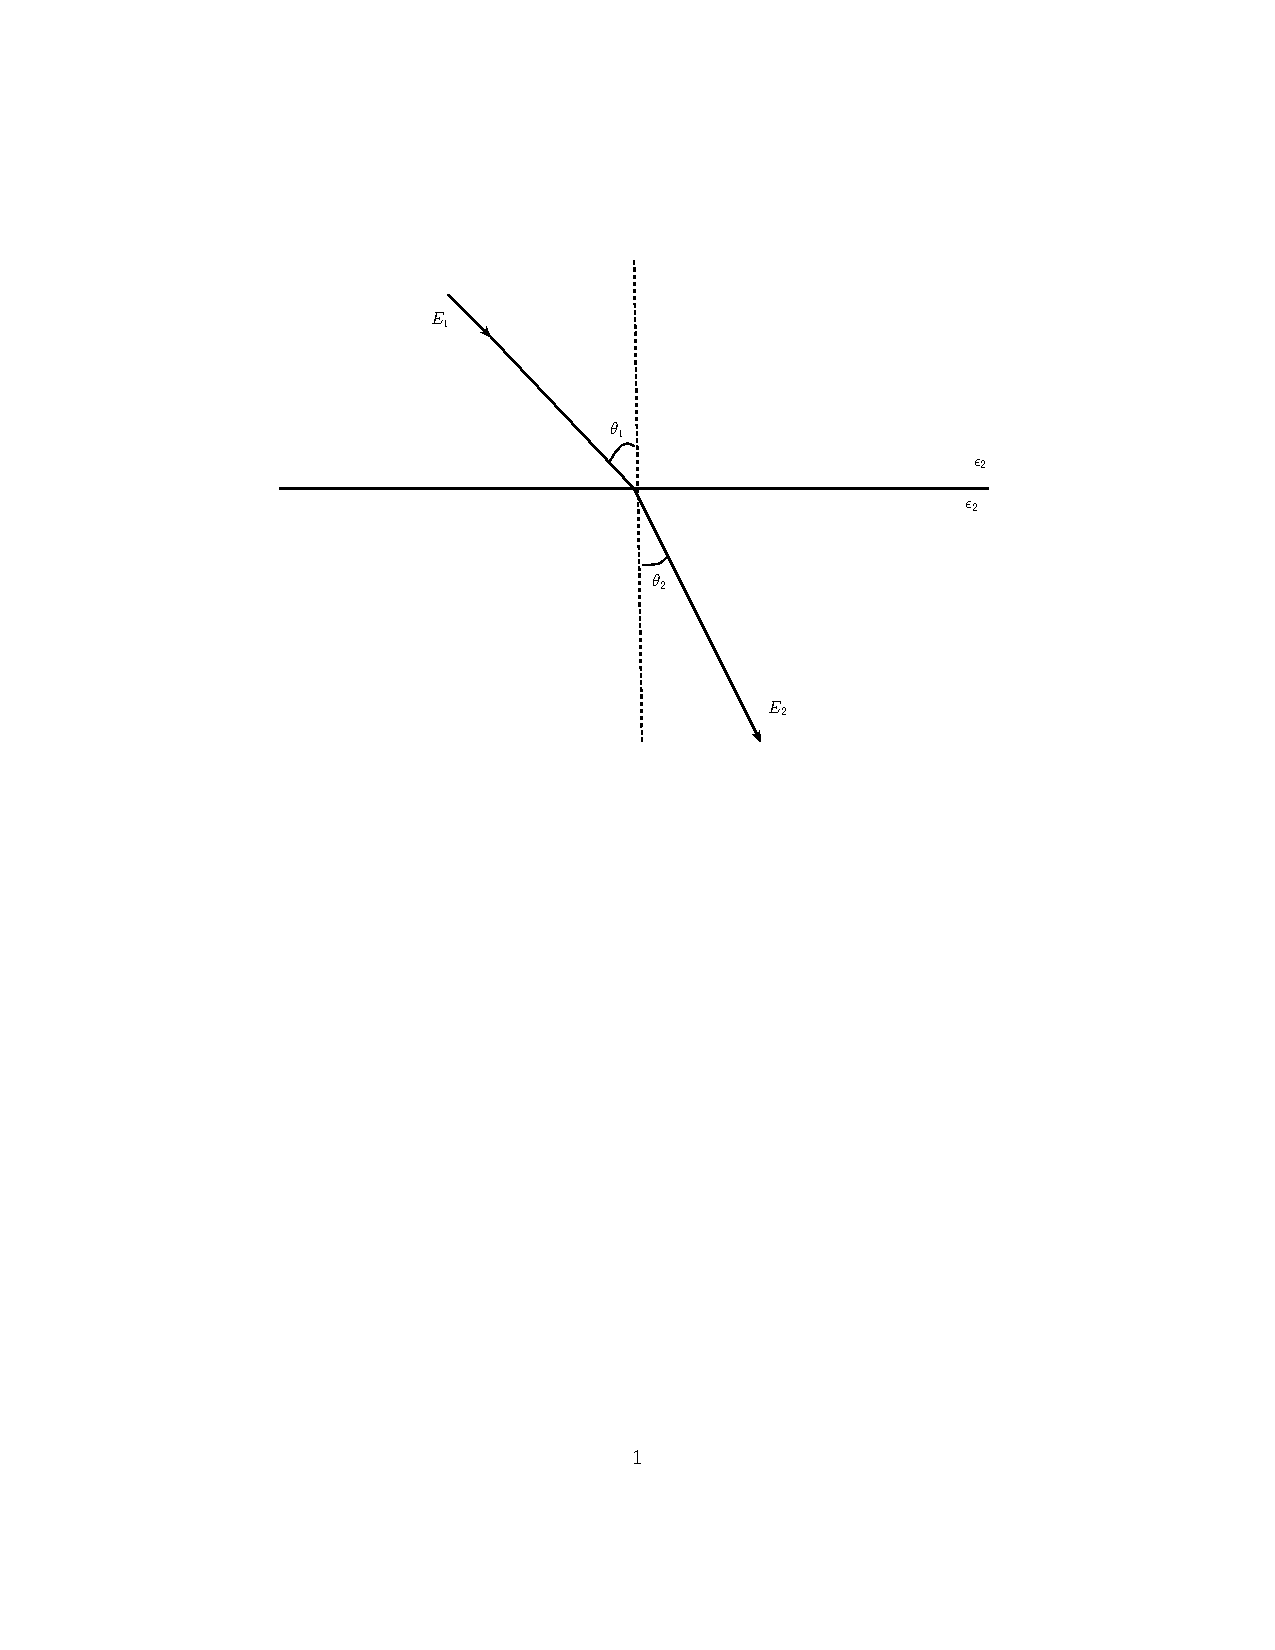
\includegraphics[width=0.7\linewidth]{figs/fig13/fig13.pdf}
			\end{minipage}
			\end{figure}
			\vspace{-200pt}


		\begin{enumerate}
			\item $\epsilon_1 \sin{\theta_1}=\epsilon_2 \sin{\theta_2}$
			\item $\epsilon_1 \cos{\theta_1} = \epsilon_2 \cos{\theta_2}$
			\item $\epsilon_1 \tan{\theta_1} = \epsilon_2 \tan{\theta_2}$
			\item $\epsilon_1 \cot{\theta_1} = \epsilon_2 \cot{\theta_2}$
		\end{enumerate}
\end{enumerate}
\end{document}


